\documentclass[../../main.tex]{subfiles}
\begin{document}

たがいに外接する定円 $C$，$C'$ が共通接線 $\ell$ の同じ側にあるとする．
図のように
\begin{enumerate}
  \item $C$，$C'$，$\ell$ に接する円を $C_1$，
  \item $C$，$C_1$，$\ell$ に接する円を $C_2$，$\cdots$
  \item $C$，$C_{n-1}$，$\ell$ に接する円を $C_n$，$\cdots$
\end{enumerate}
とする．
このとき円 $C_n$ の半径を $r_n$ として，極限値 $\displaystyle\lim_{n\to\infty}n^2r_n$ を，
円 $C$ の半径 $R$ と円 $C'$ の半径 $R'$ とを用いてあらわせ．

\begin{figure}[htbp]
  \centering
  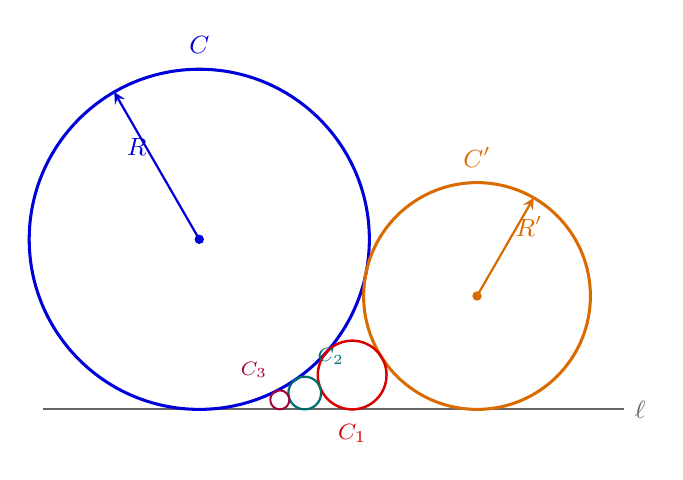
\begin{tikzpicture}[x=1.8cm, y=1.8cm, >=stealth, every node/.style={font=\small}]
    \draw[thick, gray!80!black] (-0.3, 0) -- (3.8, 0) node[right] {$\ell$};

    % 定数 R=1.2, R'=0.8
    \def\R{1.2}
    \def\Rp{0.8}
    % x 座標: C の中心を (0.8, R) とする
    \def\xC{0.8}
    \pgfmathsetmacro{\xCp}{\xC + 2.0 * sqrt(\R * \Rp)}
    \pgfmathsetmacro{\rOne}{1.0 / pow(1.0/sqrt(\R) + 1.0/sqrt(\Rp), 2)}
    \pgfmathsetmacro{\xCone}{\xC + 2.0 * sqrt(\R * \rOne)}
    \pgfmathsetmacro{\rTwo}{1.0 / pow(2.0/sqrt(\R) + 1.0/sqrt(\Rp), 2)}
    \pgfmathsetmacro{\xCtwo}{\xC + 2.0 * sqrt(\R * \rTwo)}
    \pgfmathsetmacro{\rThree}{1.0 / pow(3.0/sqrt(\R) + 1.0/sqrt(\Rp), 2)}
    \pgfmathsetmacro{\xCthree}{\xC + 2.0 * sqrt(\R * \rThree)}

    \coordinate (O) at (\xC, \R);
    \coordinate (Op) at (\xCp, \Rp);
    \coordinate (C1) at (\xCone, \rOne);
    \coordinate (C2) at (\xCtwo, \rTwo);
    \coordinate (C3) at (\xCthree, \rThree);

    % 円 C
    \draw[line width=1.1pt, blue!85!black] (O) circle (\R);
    \node[circle, fill=blue!85!black, inner sep=1.2pt] at (O) {};
    \draw[->, thick, blue!85!black] (O) -- +(120:\R) node[midway, above left] {$R$};
    \node[above=2pt, blue!85!black] at (\xC, {2*\R}) {$C$};

    % 円 C'
    \draw[line width=1.1pt, orange!85!black] (Op) circle (\Rp);
    \node[circle, fill=orange!85!black, inner sep=1.2pt] at (Op) {};
    \draw[->, thick, orange!85!black] (Op) -- +(60:\Rp) node[midway, above right] {$R'$};
    \node[above=2pt, orange!85!black] at (\xCp, {2*\Rp}) {$C'$};

    % 小円 C1, C2, C3
    \draw[line width=0.9pt, red!85!black] (C1) circle (\rOne);
    \node[below=2pt, red!85!black, font=\footnotesize] at (\xCone, 0) {$C_1$};

    \draw[line width=0.8pt, teal!85!black] (C2) circle (\rTwo);
    \node[above right=1pt, teal!85!black, font=\scriptsize] at (\xCtwo, {2*\rTwo}) {$C_2$};

    \draw[line width=0.7pt, purple!85!black] (C3) circle (\rThree);
    \node[above left=1pt, purple!85!black, font=\scriptsize] at (\xCthree, {2*\rThree}) {$C_3$};
  \end{tikzpicture}
  \caption{共通接線 $\ell$ に接する円群}
  \label{fig:problem_circles}
\end{figure}

\end{document}
